%%%%%%%%%%%%%%%%%%%%%%%%%%%%%%%%%%%%%%%%%%%%%%%%%%%%%%%%
%%%%%%%%%%%%%%%%%%%%%%%%%%%%%%%%%%%%%%%%%%%%%%%%%%%%%%%%
\section[Pheno]{Feasibility study for a search of a \Tp~at LHC at 8 TeV}
\setcounter{tocdepth}{2}

\begin{frame}
\begin{center}
Feasibility study for a search of a \Tp~at LHC at 8 TeV
\end{center}
\begin{textblock}{50}(5,90)
\textcolor{red}{PHENO}
\end{textblock}
\end{frame}

\subsection{PHENO}


\begin{frame}{Motivation - Samples - Strategy}
\vspace{-1.0cm}

\begin{center}
  \includegraphics[width=1.0\textwidth]{TprimeDecay.png}
\end{center}

\vspace{-.5cm}
\begin{columns}
\begin{column}{.60\textwidth}
%\begin{center}
\resizebox{\textwidth}{!}{
\begin{tabular}{||l|c|r||}
  \hline\hline
  Process & $\sigma_{\rm 8 TeV}$ (pb) & Expected Events (20 fb$^{-1}$) \\ \hline
 Signal ($T'j$) & 0.2 & 700 \\
 \hline
  QCD (bbjjj) & 500 & 10,000,000 \\
  \W+jets & 37,509 & 750,180,000 \\
  \Z+jets & 3,503.71 & 70,074,200 \\
  \ttbar & 234 & 4,680,000 \\
  single-$t$ & 114.85 & 2,297,000 \\
  Di-boson & 96.82 & 1,936,400 \\
  \hline\hline
\end{tabular}
}
%\end{center}
\end{column}
\begin{column}{.40\textwidth}
\begin{block}{}\tiny
Full hadronic channel $\to$ $M(5j)$:
  \begin{itemize}\tiny
  \item Huge backgrounds
  \item Highest number of expected signal events
  \end{itemize}
\textit{Study performed at hadronization level: AK5 jets}
\end{block}
\end{column}
\end{columns}

\begin{textblock}{50}(5,90)
\textcolor{red}{PHENO}
\end{textblock}

\end{frame}

\begin{frame}{Selection}
\vspace{-.2cm}

\begin{textblock}{35}(5,15)
\begin{block}{}
\tiny{
Criteria: $\sim$90\% eff $\times$ cut on signal\\
Massive \Tp~$\to$ boosted top-Higgs\\
\textbf{Cut 0}: $N(j)[|\eta|<2.5]\ge 6$\\  
\hspace{.6cm} $N(j)[2<|\eta|<5]\ge 1$\\
\textbf{Cut 1}: 
\begin{tabular}{|c|c|}
  \hline
  \pt & $>$ [GeV/c] \\ 
  \hline
  $j_{1}$ & 150 \\
  $j_{2}$ & 80 \\
  $j_{3}$ & 60 \\
  $j_{4}$ & 60 \\
  \hline
\end{tabular}\\
\textbf{Cut 2}: $H_{T}>630$~GeV/c\\
\hspace{.6cm} with $H_{T}=\sum |p_{T}(j)|$\\
\textbf{Cut 3}: $N(b)\ge 2$\\
\textbf{Cut 4}: $\Delta R(bb)< 1.8$\\
\textbf{Cut 5}: $p_{T}(H)>200$~GeV/c\\
\hspace{.6cm} $p_{T}(t)>300$~GeV/c\\
\textbf{Cut 6}: $2.2<\Delta R_{HW}<3.5$\\
\textbf{Cut 7}: $\Delta \phi_{H(bb)}<2.0$\\
\hspace{.6cm} $\Delta \phi_{top(bW)}<3.3$\\
\textbf{Cut 8}: $\Delta \phi_{W(jj)}<2.3$\\
\textbf{Cut 9}: $100$~\GeVcc $<M(bb)<135$~\GeVcc\\
\textbf{Cut 10}: $\frac{p_{T}^{H}+p_{T}^{t}}{H_{T}}>0.65$\\
%\textbf{Cut 10}: \\
%\textbf{Cut 5}: 
}%
\end{block}
\end{textblock}

\begin{textblock}{35}(45,17)
    \includegraphics[width=1.0\textwidth]{SixthJet.png}
\end{textblock}
\begin{textblock}{35}(85,15)
    \includegraphics[width=1.0\textwidth]{HT.png}
\end{textblock}
\begin{textblock}{80}(45,50)
    \includegraphics[width=1.0\textwidth]{HPTTPT.png}
\end{textblock}


\begin{textblock}{50}(5,90)
\textcolor{red}{PHENO}
\end{textblock}

\end{frame}



\begin{frame}{Results}
\vspace{-2.5cm}

\begin{columns}
\begin{column}{.50\textwidth}
\begin{block}{}\scriptsize
Number of events in a window of $20$~GeV around $M(T')=734$ \GeVcc\\
\vspace{1.0cm}
\centering{
\textbf{
$\frac{S}{B}=0.06\pm 0.02$: S is 6\% of B\\
$\frac{S}{\sqrt{S+B}}=2.0\pm 0.3$: Significance of 2}}
%\begin{equation*}                                               
%\frac{S}{B}=0.06\pm 0.02\; \mbox{and} \; \frac{S}{\sqrt{S+B}}=2.0\pm 0.3                                           
%\end{equation*}
\end{block}
\end{column}

\begin{column}{.50\textwidth}
\begin{figure}[!Hhtbp]
  \begin{center}
    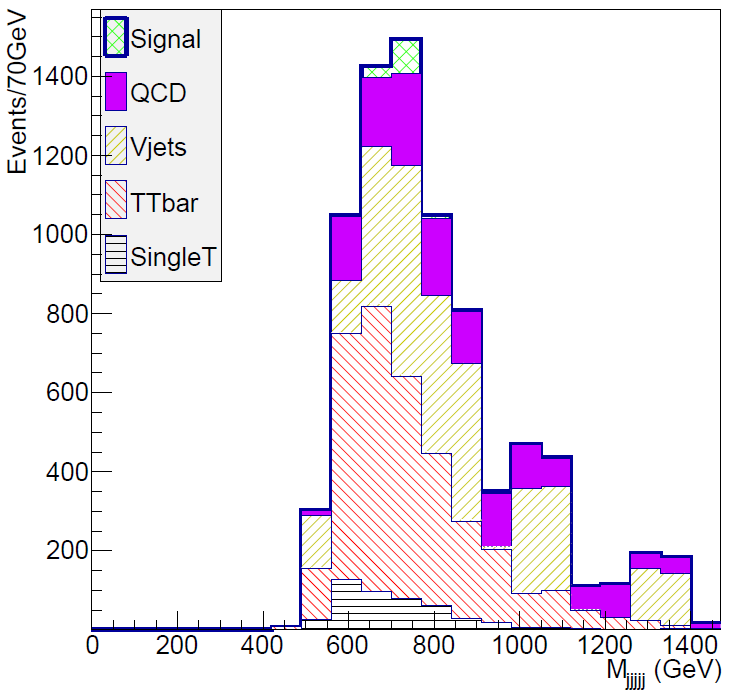
\includegraphics[width=1.0\textwidth]{../figs/Pheno/Final.png}
    %\caption{Reconstructed \Tp~mass after all cuts for backgrounds and signal (stacked) normalized to 20~$fb^{-1}$ luminosity. Signal peak is visible on top of the sum of backgrounds.}
    %\label{fig:M5J}
  \end{center}
\end{figure}
\end{column}
\end{columns}


\begin{textblock}{75}(50,67)
\resizebox{\textwidth}{!}{
\begin{tabular}{l|c|c|c|c}
 & \multicolumn{2}{c|}{unweighted events}  & \multirow{2}{*}{weight} & weighted  \\
 & after Cut 10 & in mass window & & events \\
 \hline
 Signal & $8601$ & $3780$ & $0.018$ &$69 \pm 1$ \\
 \hline
   $t \bar{t}$ & $409$ & $57$ & $7.7$ & $437 \pm 58$ \\
 $W$+jets & $24$ & $3$ & $132$ & $395 \pm 228$ \\
 $QCD$ & $235$ & $34$ & $6.48$ & $220 \pm 38$ \\
 $tW$ & $18$ & $3$ & $11.3$ & $34 \pm 20$ \\
 $t$+ jet & $75$ & $7$ & $3.55$ & $25 \pm 9$ \\
  \hline
  total background & & & & $1112 \pm 352$ \\
\end{tabular}
}
\end{textblock}

\begin{textblock}{50}(5,90)
\textcolor{red}{PHENO}
\end{textblock}

\begin{textblock}{43}(4,55)
\begin{alertblock}{}\tiny
\textcolor{red}{Strong motivation for a data analysis!}\\
Work done with theoreticians: \\\textbf{Aldo Deandrea and Giacomo Cacciapaglia}\\
\textbf{1 proceedings}: Les Houches 2013: Physics at TeV Colliders: New Physics Working Group Report \textbf{arXiv:1405.1617} \\
\textbf{1 paper}: Fully hadronic decays of a singly produced vectorlike top partner at the LHC \textbf{Phys.Rev. D90 (2014) 11, 115008}
\end{alertblock}
\end{textblock}

\end{frame}

%%%%%%%%%%%%%%%%%%%%%%%%%%%%%%%%%%%%%%%%%%%%%%%%%%%%%%%%%%%%%%%%%%%%%%%%%%%%%%%%%%%%%%%%%%%%%%%%%%%%%%%%%%%%%%%%%%%%%%%%%%%%%

\iffalse
\begin{frame}{Motivation - Samples - Strategy}
\vspace{-.5cm}

\begin{columns}
\begin{column}{.50\textwidth}
\begin{block}{Motivation}
\begin{itemize}\tiny
\item Single produced \Tp~with mixings to light quark generations $\to$ Enhanced production cross section
\item Full hadronic channel:
  \begin{itemize}\tiny
  \item Difficult $\to$ huge backgrounds
  \item Highest number of expected events
  \item It is possible to reconstruct the \Tp~mass
  \item It needs techniques to choose the jets to reconstruct the \Tp
  \end{itemize}
\item $T'\to tH, tZ, bW$ and $Br(T'\to tH)=0.5$ $Br(H\to b\bar{b})=0.57$ $Br(t\to bq\bar{q}')=0.66$
\end{itemize}
\end{block}
\end{column}

\begin{column}{.50\textwidth}
%\begin{table}[htbH]
\begin{center}
\resizebox{\textwidth}{!}{
\begin{tabular}{||l|c|r||}
  \hline\hline
  Process & $\sigma_{\rm 8 TeV}$ (pb) & Expected Events \\ \hline
 Signal ($T'j$) & 0.2 & 700 \\
 \hline
  QCD (bbjjj) & 500 & 10,000,000 \\
  \W+jets & 37,509 & 750,180,000 \\
  \Z+jets & 3,503.71 & 70,074,200 \\
  \ttbar & 234 & 4,680,000 \\
  single-$t$ & 114.85 & 2,297,000 \\
  Di-boson & 96.82 & 1,936,400 \\
  \hline\hline
\end{tabular}
}
%\caption{Cross sections and expected number of events for background processes and signal for a luminosity of 20~$fb^{-1}$. \label{tab:xsec}}
\end{center}
%\end{table}
\vspace{-.5cm}
\begin{block}{}
\tiny $M(5j)$ $\to$ Five jets invariant mass as variable of interest
\end{block}
\end{column}
\end{columns}

\vspace{-.2cm}
\begin{block}{Strategy}
\begin{itemize}\tiny
\item Signal: 3 $b$-quarks and 2 light quarks $\to$ High b-jet multiplicity
\item Real Higgs boson and top quark in signal events
\item Method to have a good identification of the 5 jets coming from the \Tp:
\begin{itemize}\tiny
\item Tag b--jets and keep events with at least two.
\item b-jets pairs used to reconstruct the Higgs boson $\to$ ${\Delta R_{bb} <2.5}$ and pair with closest mass to the Higgs boson mass (125~\GeVcc)
\item b-jets removed from jets collection $\to$ jets pair with closest mass to the W-mass (80~\GeVcc) chosen to reconstruct the \W~boson 
\item Higgs and \W~boson jets removed from jet collection $\to$ the jet giving the closest mass to the top mass (172~\GeVcc), combined with W-jets, was used to reconstruct the top quark
\end{itemize}
\end{itemize}

\end{block}

\end{frame}

\begin{frame}{Selection}
\vspace{-.2cm}

\begin{columns}
\begin{column}{.50\textwidth}
\begin{block}{}
\begin{itemize}\scriptsize
\item \textit{Cut 0}: At least 6 jets with ${p_T > 30}$~GeV/c are required. At least five jets within $|\eta|<2.5$ and at least one jet within $2<|\eta|<5$. The \Tp~decays into five central jets. One associated jet in the forward direction. \\
\textbf{Figure}: $\eta$ distribution of the forward jet produced in association with \Tp. Signal sample is normalized to theoretical cross section and to 20~$fb^{-1}$.
\item \textit{Cut 1}: ${p_{T}(j_{1})>150}$~GeV/c, ${p_{T}(j_{2})>80}$~GeV/c, ${p_{T}(j_{3,4})>60}$~GeV/c
\item \textit{Cut 2}: $H_{T}>630$~GeV/c with $H_{T}=\sum |p_{T}(j)|$\\
\textbf{Figure}: Total hadronic energy for backgrounds (stacked) and signal (over--imposed) normalized to 20~$fb^{-1}$ luminosity. $H_{T}$ is higher in signal than in background events.
\end{itemize}
\end{block}
\end{column}

\begin{column}{.50\textwidth}
\begin{figure}[!Hhtbp]
  \begin{center}
    \includegraphics[width=0.75\textwidth]{../figs/Pheno/SixthJet.png}\\
    \includegraphics[width=0.75\textwidth]{../figs/Pheno/HT.png}
  \end{center}
\end{figure}
\end{column}
\end{columns}

\end{frame}

\begin{frame}{}
\vspace{-.2cm}

\begin{columns}
\begin{column}{.50\textwidth}
\begin{block}{}
\begin{itemize}\scriptsize
\item \textit{Cut 3}: At least two b-jets with effective CSV algorithm with medium working point
\item \textit{Cut 4}: Events with a Higgs candidate with $p_{T}>200$~GeV/c and a top candidate with $p_{T}>300$~GeV/c\\
\textbf{Figure}: Reconstructed Higgs candidate $p_{T}$ in the x axis and reconstructed top candidate $p_{T}$ in the y axis for backgrounds (left) and signal (right). Signal events have reconstructed Higgs and top with higher \pt~than backgrounds.
\item \textit{Cut 6}: Events with $2.2<\Delta R_{HW}<3.5$ were kept\\
\textbf{Figure}: $\Delta R$ between the reconstructed Higgs and \W~candidates for backgrounds (stacked) and signal (over--imposed) normalized to 20 $fb^{-1}$ luminosity. However signal and backgrounds have a mean value of $\Delta R_{HW}=3$, backgrounds tend to have lower values than signal, as well as larger tails.
\end{itemize}
\end{block}
\end{column}

\begin{column}{.50\textwidth}
\begin{figure}[!Hhtbp]
\begin{center}
\includegraphics[width=1.0\textwidth]{../figs/Pheno/HPTTPT.png}\\
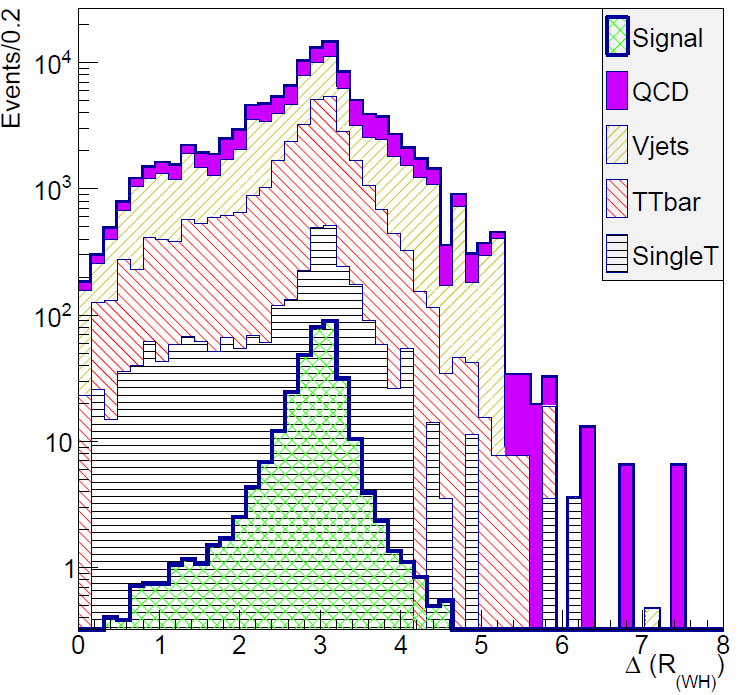
\includegraphics[width=0.75\textwidth]{../figs/Pheno/DRWH.png}
\end{center}
\end{figure}
\end{column}
\end{columns}

\end{frame}

\begin{frame}{}
\vspace{-.2cm}

\begin{columns}
\begin{column}{.50\textwidth}
\begin{block}{}
\begin{itemize}\scriptsize
\item \textit{Cut 7}: Events with $\Delta \phi_{H(bb)}<2.0$ and $\Delta \phi_{top(bW)}<3.3$ were kept
\item \textit{Cut 8}: Events were required to have $\Delta \phi_{W(jj)}<2.3$ 
\item \textit{Cut 9}: Events with a Higgs candidate with a mass between $100$~\GeVcc~and $135$~\GeVcc~were selected\\
\textbf{Figure}: Mass of the reconstructed Higgs candidate for backgrounds (stacked) and signal (over--imposed). Backgrounds have larger tails than signal for the reconstructed Higgs mass.
\item \textit{Cut 10}: Events with $\frac{p_{T}^{H}+p_{T}^{t}}{H_{T}}>0.65$ were kept\\
\textbf{Figure}: Relative total hadronic energy for backgrounds (stacked) and signal (over--imposed) normalized to 20 $fb^{-1}$ luminosity.
\end{itemize}
\end{block}
\end{column}

\begin{column}{.50\textwidth}
\begin{figure}[!Hhtbp]
  \begin{center}
    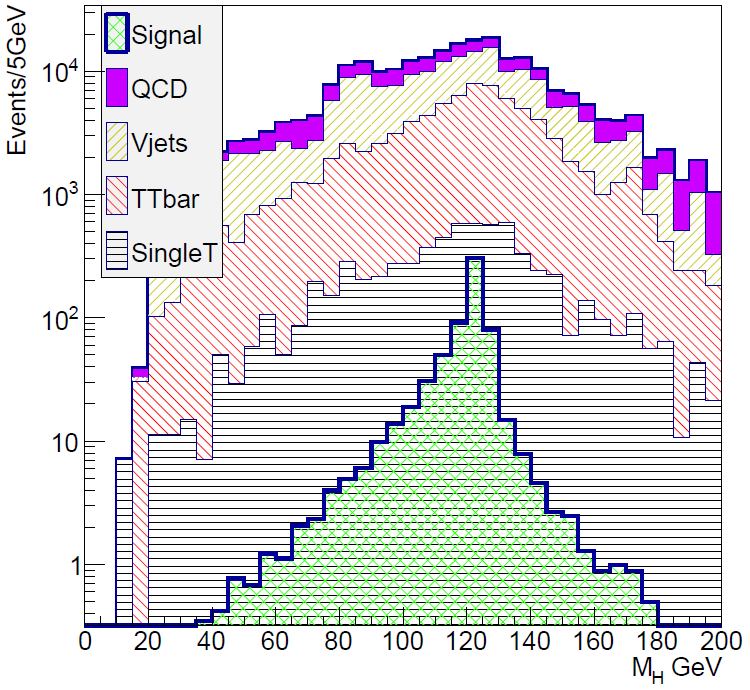
\includegraphics[width=0.75\textwidth]{../figs/Pheno/MH.png}\\
    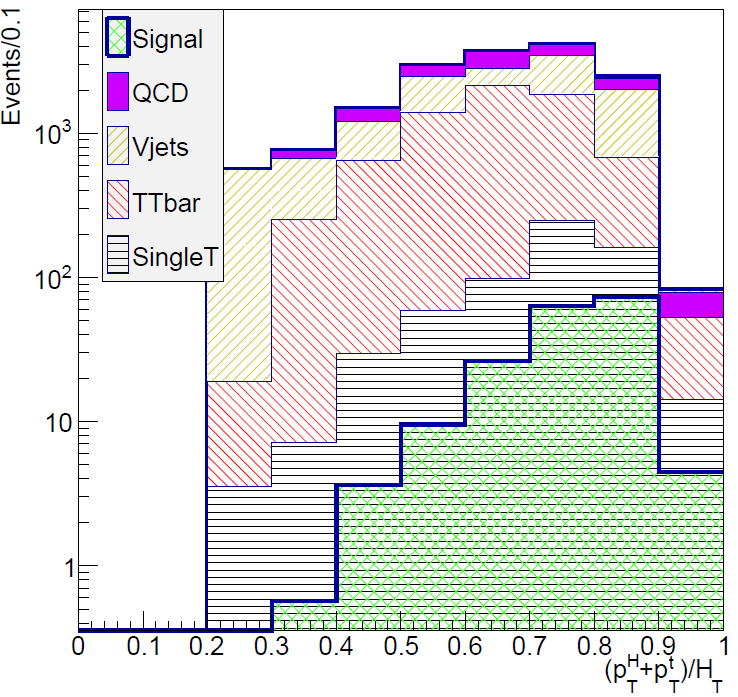
\includegraphics[width=0.75\textwidth]{../figs/Pheno/RelHT.png}
  \end{center}
\end{figure}
\end{column}
\end{columns}

\end{frame}

\begin{frame}{Results}
\vspace{-.2cm}

\begin{columns}
\begin{column}{.50\textwidth}
\begin{block}{}\scriptsize
The number of events falling into a window of $20$~GeV around the \Tp~mass ($M(5j)$) were selected [$M(T')=734$ \GeVcc~in the signal MC sample used]\\
\textbf{Figure}: Reconstructed \Tp~mass after all cuts for backgrounds and signal (stacked) normalized to 20~$fb^{-1}$ luminosity. Signal peak is visible on top of the sum of backgrounds.

\begin{center}
\resizebox{\textwidth}{!}{
\begin{tabular}{l|c|c|c|c}
 & \multicolumn{2}{c|}{unweighted events}  & \multirow{2}{*}{weight} & weighted  \\
 & after Cut 10 & in mass window & & events \\
 \hline
 Signal & $8601$ & $3780$ & $0.018$ &$69 \pm 1$ \\
 \hline
   $t \bar{t}$ & $409$ & $57$ & $7.7$ & $437 \pm 58$ \\
 $W$+jets & $24$ & $3$ & $132$ & $395 \pm 228$ \\
 $QCD$ & $235$ & $34$ & $6.48$ & $220 \pm 38$ \\
 $tW$ & $18$ & $3$ & $11.3$ & $34 \pm 20$ \\
 $t$+ jet & $75$ & $7$ & $3.55$ & $25 \pm 9$ \\
  \hline
  total background & & & & $1112 \pm 352$ \\
\end{tabular}
}
%\caption{Number of signal and background events from utilized MC samples: in the first column the simulated events that pass all kinematic cuts, in the second column the events that fall in the mass window ${710<M_{jjjjj}<750}$~\GeVcc, finally in the fourth column the number of weighted events in the mass window normalized to the physical cross section (the applied weight is listed in the third column). All the errors are statistical only. For the total background, the linear sum of errors was considered.} \label{tab:events}
\end{center}

Discriminators:
\begin{equation*}                                               
\frac{S}{\sqrt{S+B}}=2.0\pm 0.3\, \mbox{and} \, \frac{S}{B}=0.06\pm 0.02                                               
\end{equation*}
\end{block}
\end{column}

\begin{column}{.50\textwidth}
\begin{figure}[!Hhtbp]
  \begin{center}
    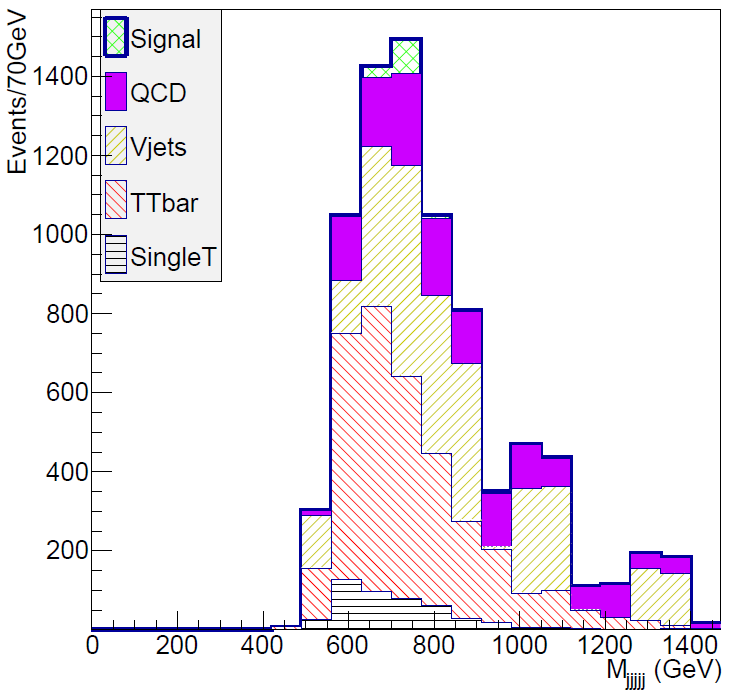
\includegraphics[width=1.0\textwidth]{../figs/Pheno/Final.png}
    %\caption{Reconstructed \Tp~mass after all cuts for backgrounds and signal (stacked) normalized to 20~$fb^{-1}$ luminosity. Signal peak is visible on top of the sum of backgrounds.}
    %\label{fig:M5J}
  \end{center}
\end{figure}
\end{column}
\end{columns}

\end{frame}

\fi

%\begin{frame}{}
%\vspace{-.2cm}
%
%\begin{columns}
%\begin{column}{.50\textwidth}
%\begin{block}{}
%\begin{itemize}\scriptsize
%\item 
%\end{itemize}
%\end{block}
%\end{column}
%
%\begin{column}{.50\textwidth}
%
%\end{column}
%\end{columns}
%
%\end{frame}
